\begin{figure}[h]
    \centering
    \begin{subfigure}[b]{0.48\textwidth}
        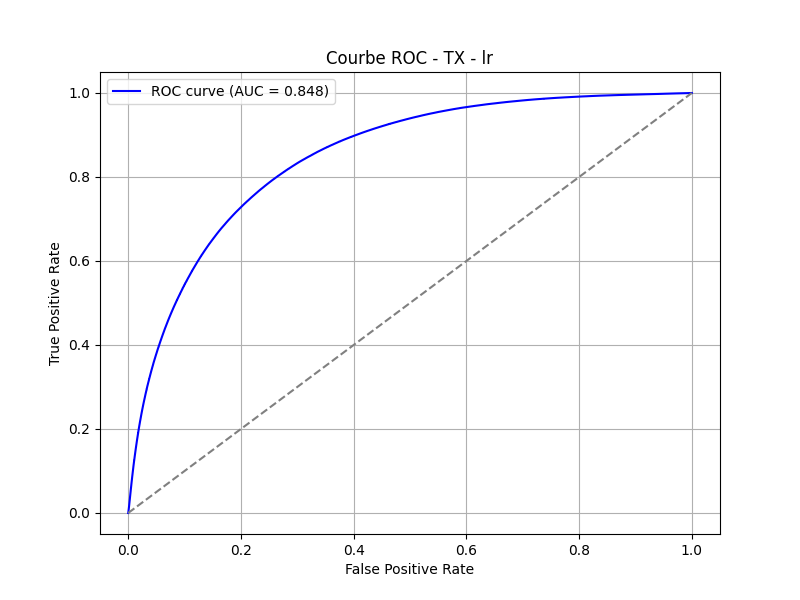
\includegraphics[width=\textwidth]{Images/curve_roc_folktables/roc_curve_TX_lr.png}
        \caption{Curve ROC (AUC = 0.848): model = Logistic Regression}
        \label{fig:TX_lr}
    \end{subfigure}
    \hfill
    \begin{subfigure}[b]{0.48\textwidth}
        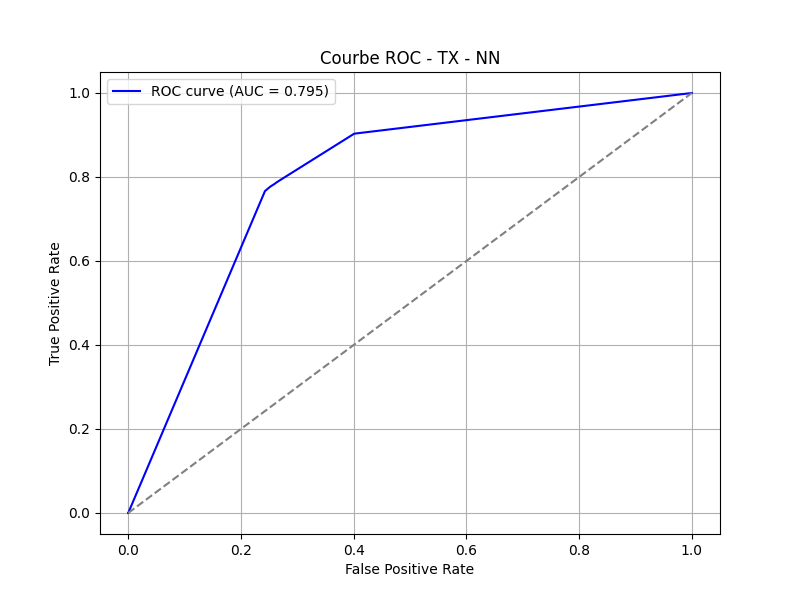
\includegraphics[width=\textwidth]{Images/curve_roc_folktables/roc_curve_TX_NN.png}
        \caption{Curve ROC (AUC = 0.795): model = Neural Network}
        \label{fig:TX_nn}
    \end{subfigure}

    \begin{subfigure}[b]{0.48\textwidth}
        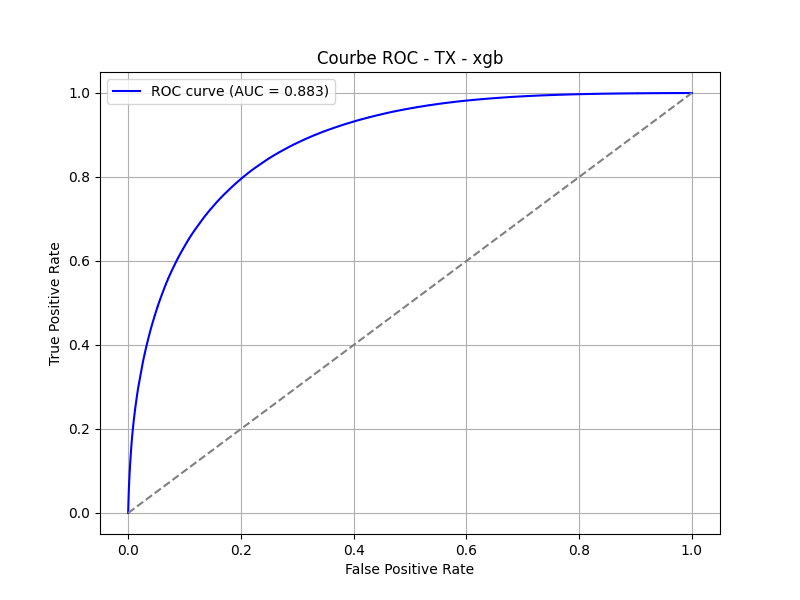
\includegraphics[width=\textwidth]{Images/curve_roc_folktables/roc_curve_TX_xgb.png}
        \caption{Curve ROC (AUC = 0.883): model = XGBoost}
        \label{fig:TX_xgb}
    \end{subfigure}
    \hfill
    \begin{subfigure}[b]{0.48\textwidth}
        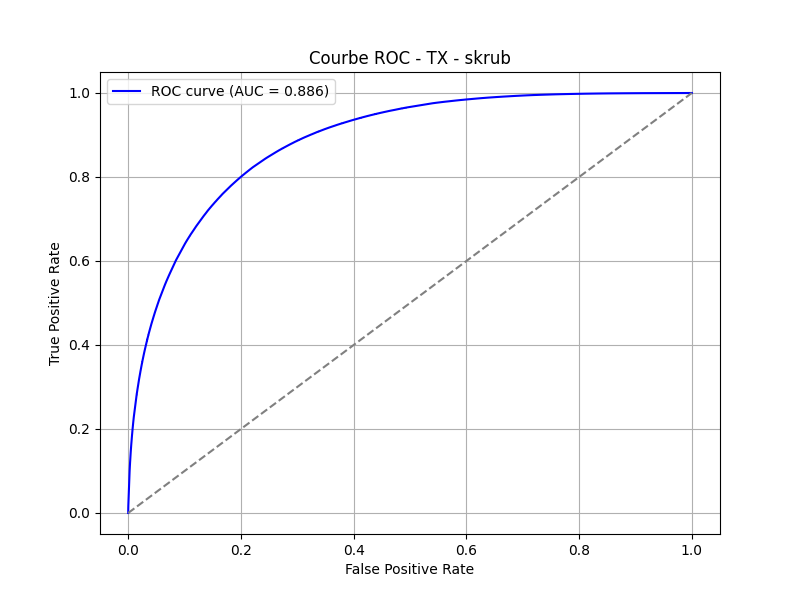
\includegraphics[width=\textwidth]{Images/curve_roc_folktables/roc_curve_TX_skrub.png}
        \caption{Curve ROC (AUC = 0.886): model = HistGradientBoosting}
        \label{fig:TX_skrub}
    \end{subfigure}
    \caption{Comparison of the models trained on the sub dataset of the Texas state}
    \label{fig:roc_tx}
\end{figure}